% !TeX root = ..//diffgeo_main.tex

\begin{figure}[H]
\centering
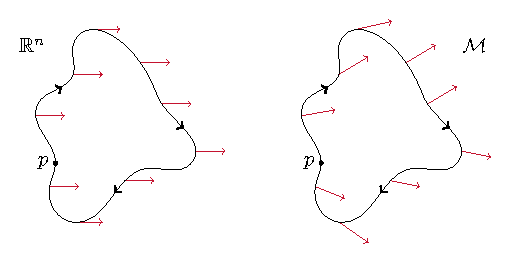
\includegraphics[width=0.7\linewidth]{figures/tikz/parallelshift_rn_vs_manifold.pdf}
\label{img:parallelshift_rn_vs_manifold}
\caption{Parallelverschiebung auf Kurve $c$ in $\R^n$ vs. auf beliebiger Mannigfaltigkeit $\mfk$}
\end{figure} 

Die kovariante Ableitung lässt sich durch Parallelverschiebung ausdrücken.
Wir bezeichnen die Parallelverschiebung entlang $c$ mit $P_c$, wobei $c: (-\epsilon , \epsilon) \to \mfk$ eine Kurve in $\mfk$ ist.
\begin{figure}[H]
\centering
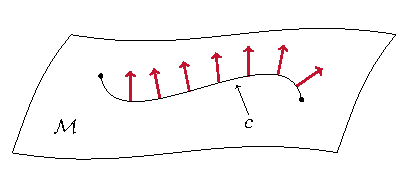
\includegraphics[width=0.5\linewidth]{figures/tikz/parallel_shift_on_curve.pdf}
\label{img:parallel_shift_on_curve}
\end{figure} 
Es gelte $c(0)=p$, $c'(0) = X_p$ und $Y$ sei ein glattes Vektorfeld auf $\mfk$.
Dann gilt:

\begin{align}
\label{eq:parallelcovd}
\nabla_{X_p} Y = \lim\limits_{t \rightarrow 0} \frac{1}{t} \left( P^{-1}_{c(t)} Y_{c(t)} - Y_p\right) 
\end{align}

\begin{bew}[Beweis von Gleichung \ref{eq:parallelcovd}]
Für $Y$, definiert in einer Umgebung von $p_y$, ist der Wert $(\nabla_X Y)(p)$ vollständig bestimmt durch Restriktion von $Y$ auf die Kurve $c$ mit $c'(0) = X_p$.
Expandiere $Y$ als Linearkombination paralleler Vektorfelder längs $c$.

Sei $\{ \hat{w}_1, \dots, \hat{w}_n \}$ eine Basis von $T_p \mfk$.
Sei $w_i : (-\epsilon, \epsilon) \to \mfk$ das parallele Vektorfeld längs $c$ mit $w_i(0) = \hat{w}_i$.
Mit anderen Worten  $\{ w_1(t), \dots, w_n (t)\}$st eine Basis von $T_{c(t)}\mfk$.
\begin{align}
Y = \sum^m_{i=1} a_i w_i
\end{align}
Mit Koeffizienten $a_i: (-\epsilon , \epsilon) \to \R$.\\
Betrachte:
\begin{align}
\lim\limits_{t \rightarrow 0} \frac{1}{t} \left( P^{-1}_{c(t)} Y(t) - Y(0)\right) &=  \lim\limits_{t \rightarrow 0} \frac{1}{t} \left( \sum^m_{i=1} (a_i (t) - a_i (0)) \cdot w_i (0) \right)\\
&= \sum^m_{i=1} \left( \dv{t} a_i (t) \right) \eval_{t=0} w_i (0)\\
&= \covd_t \left( \sum^m_{i=1} a_i w_i \right) \eval_{t=0}\\
&= \nabla_X Y
\end{align}
\end{bew}

\begin{defs}[Parallele Fortsetzung]
Sei $p \in \mfk$ und $v \in T_p \mfk$, dann existiert ein paralleles Vektorbündel längs $c$ mit $X\eval_p = v$.\\
$X\eval_p$ heißt parallele Fortsetzung von $v$.
\end{defs}
Es sellt sich nun die folgende Frage:\\
\textit{Kann man $v \in T_p \mfk$ zu einem parallelen Vektorfeld in einer Umgebung von $p$ fortsetzen?
Also existiert ein Vektorfeld $X$ auf $\mfk$ in einer Umgebung $U$ von $p$, sodass $X\eval_p = v$ und $X$ parallel sind?}
\begin{figure}[H]
\centering
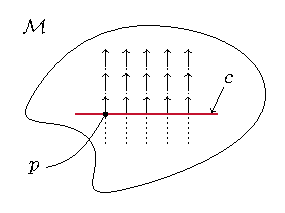
\includegraphics[width=0.6\linewidth]{figures/tikz/parallel_transport.pdf}
\label{img:parallel_transport}
\caption{Paralleltransport}
\end{figure} 
Gegeben sei 
\begin{align}
V: [0, 1] \times [0, 1] \to \mfk\\
(t, \tau) \mapsto V(t, \tau)
\end{align}
Damit erhalten wir ein Vektorfeld $Z$ in einer Umgebung von $p$:
\begin{align}
\label{eq:vectorfieldz}
\nabla_{\pdv{t}} Z \eval_{(t, 0)} = 0, \quad \nabla_{\pdv{\tau}} Z = 0
\end{align}
Wir hätten gerne, dass $\nabla_{\pdv{t}} Z = 0$.
Es genügt zu zeigen, dass folgendes gilt:
\begin{align}
\nabla_{\pdv{\tau}}\nabla_{\pdv{t}} Z = 0
\end{align}
\ref{eq:vectorfieldz} impliziert:
\begin{align}
\nabla_{\pdv{t}}\nabla_{\pdv{\tau}} Z = 0
\end{align}
Es muss deshalb zwangsweise gelten:
\begin{align}
\nabla_{\pdv{t}}\nabla_{\pdv{\tau}} Z - \nabla_{\pdv{\tau}}\nabla_{\pdv{t}} Z = 0.
\end{align}
Da $\comm{\pdv{\tau}}{\pdv{t}} = 0$ gilt, ist 
\begin{align}
\curv \left( \pdv{\tau}, \pdv{t} \right) Z = 0
\end{align} 
Das bedeutet also falls $\nabla_{\pdv{t}}Z = 0$, dann gilt $\curv = 0$.
Mit anderen Worten $\curv = 0$ ist eine notwendige Bedingung für die Parallelität.
Man kann zeigen, dass $\curv \equiv 0$ auch hinreichend ist.\\

Betrachte nun die folgende Situation:
\begin{figure}[H]
\centering
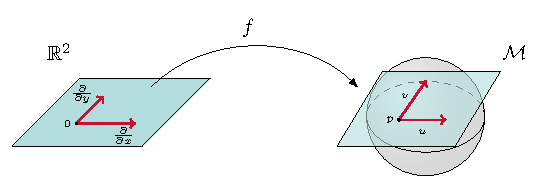
\includegraphics[width=1\linewidth]{figures/tikz/coordinates_r2_manifold.pdf}
\label{img:coordinates_r2_manifold}
\end{figure} 


Sei $f$ glatt und $f(0)=p$ und sei außerdem
\begin{align}
& \dd f \eval_0 \left( \pdv{x} \right) = f_x (0) = u\\
& \dd f \left( \pdv{y}\right) = f_y(0) = v.
\end{align}
Es sei eine Familie von Kurven $c_s$ wobei $0 \leq s \leq 1$ und $c_s (0) = c_s(1) = 0$.
\begin{figure}[H]
\centering
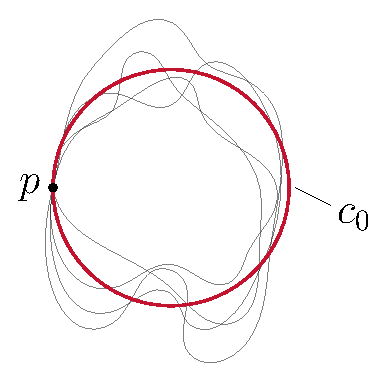
\includegraphics[width=0.4\linewidth]{figures/tikz/variantion_of_closed_curve.pdf}
\label{img:variantion_of_closed_curve}
\caption{Variation der Kurve $c_0$}
\end{figure} 

$P_s$ ist die Parallelverschiebung längs $c_s$.
Wir definieren
\begin{align}
&c : I \times I \to \mfk\\
&(s, t) \mapsto c(s,t)
\end{align}
wie folgt:
\begin{align}
c(s, t) = \left\{
\begin{array}{ll}
f(4 s t, 0) & 0 \leq t \leq \nicefrac{1}{4} \\
f(s, s(4t-1)) & \nicefrac{1}{4} \leq t \leq \nicefrac{1}{2}\\
f(s(3-4t), s) & \nicefrac{1}{2} \leq t \leq \nicefrac{3}{4}\\
f(0, 4s(1-t)) & \nicefrac{3}{4} \leq t \leq 1
\end{array}
\right. 
\end{align}
\begin{satz}
Sei $p \in \mfk$, $u$, $v \in T_p \mfk$ und $f: U \to \mfk$ sei wie oben definiert.
$P_s$ sei die Parallelverschiebung längs $c_s$ von $c_s(0) = p$ nach $c_s(1) = 0$.
Dann gilt:
\begin{align}
\partial_s \partial_s P_s(0) = 2 \curv (u, v)
\end{align}
\end{satz}

\chapter{Riemannsche Mannigfaltigkeiten}

\section{Wiederholung: Symmetrische Bilinearform}
\begin{defs}[Entartung, Index]
\begin{itemize}
\item Eine symmetrische Bilinearform $B: V \times V \to \R$ ist nicht entartet, falls:
\begin{align}
&B(v, w) = 0, \quad \forall w \in V\\
&\Rightarrow v = 0.
\end{align}
\item $\mathrm{Index}(B) = \max \{ \dim W \vert W \subset V $ ist UR mit $\dim n$ und $B\vert_{W \times W}$ ist negativ definit. $\}$
\end{itemize}
\end{defs}
Es existiert eine Basis ${b_1, \dots b_n}$ von $V_i$, so dass
\begin{align}
c(s, t) = \left\{
\begin{array}{ll}
\hphantom{-} 0 & i \neq j \\
-1 & 1\leq i \leq \mathrm{Index}(B)\\
\hphantom{-} 1 & \mathrm{Index}(B) + 1 \leq i \leq n\\
\end{array}
\right. 
\end{align}
\begin{defs}[Bilinearform zurückholen]
Seien $V$, $W$ $\R$- Vektorräume und $B_V : V \times V \to \R$ eine nicht-entartete symmetrische Bilinearform.
sei außerdem $\phi : W \to V$ eine lineare Abbildung.
Dann ist die zurückgeholte Bilinearform:
\begin{align}
(\phi^\ast B_V) (w_1, w_2) := B(\phi(w_1), \phi(w_2))
\end{align}
\end{defs}
\begin{bem}\leavevmode
\begin{itemize}
\item $(\phi^\ast B_V)$ ist eine symmetrische Bilinearform, die entartet sein kann.
\item Wenn $B_V$ positiv definit und $\phi$ injektiv ist, dann folgt daraus, dass $(\phi^\ast B_V)$ positiv definit ist.
\end{itemize}
\end{bem}

\begin{defs}[Isometrie]
Seien $V$, $W$ $\R$- Vektorräume mit nicht-entarteten Bilinearformen $B_V$ und $B_W$.
$\phi: W \to V$ heißt Isometrie, falls $(\phi^\ast B_V) = B_W$.
\end{defs}

\section{Riemannsche Metriken}

\begin{defs}[Riemannsche Metriken]
Eine (Semi- ) Riemannsche Metrik auf einer differenzierbaren Mannigfaltigkeit $\mfk$, ist eine Familie von nicht-entarteten symmetrischen Bilinearformen 
$(g_p)_{p \in \mfk}$ auf $T_p \mfk$, so dass für alle $X$, $Y$ $\in \mathfrak{X}(\mfk)$ gilt:
\begin{align}
&g_{\cdot} (X_\cdot, Y_\cdot): \mfk \to \R \\
& p \mapsto g_p (X_p, Y_p)
\end{align}
ist glatt in $p \in \mfk$.
\end{defs}


\begin{bem}\leavevmode
\begin{itemize}
\item Eine solche Metrik heißt Riemannsch, wenn $g_p$ positiv definit für alle $p$ in $\mfk$.
\item Eine solche Metrik heißt Lorentz-Metrik, falls $\mathrm{Index} (g_p) = 1$ für alle $p$ in $\mfk$.
\end{itemize}
\end{bem}

\textbf{Zu Semi-Riemannsch}:
Index potentiell $\geq 1$, aber auch Riemannsche Metriken werden als Semi-Riemannsch bezeichnet.



